% Options for packages loaded elsewhere
\PassOptionsToPackage{unicode}{hyperref}
\PassOptionsToPackage{hyphens}{url}
%
\documentclass[
]{book}
\usepackage{lmodern}
\usepackage{amssymb,amsmath}
\usepackage{ifxetex,ifluatex}
\ifnum 0\ifxetex 1\fi\ifluatex 1\fi=0 % if pdftex
  \usepackage[T1]{fontenc}
  \usepackage[utf8]{inputenc}
  \usepackage{textcomp} % provide euro and other symbols
\else % if luatex or xetex
  \usepackage{unicode-math}
  \defaultfontfeatures{Scale=MatchLowercase}
  \defaultfontfeatures[\rmfamily]{Ligatures=TeX,Scale=1}
\fi
% Use upquote if available, for straight quotes in verbatim environments
\IfFileExists{upquote.sty}{\usepackage{upquote}}{}
\IfFileExists{microtype.sty}{% use microtype if available
  \usepackage[]{microtype}
  \UseMicrotypeSet[protrusion]{basicmath} % disable protrusion for tt fonts
}{}
\makeatletter
\@ifundefined{KOMAClassName}{% if non-KOMA class
  \IfFileExists{parskip.sty}{%
    \usepackage{parskip}
  }{% else
    \setlength{\parindent}{0pt}
    \setlength{\parskip}{6pt plus 2pt minus 1pt}}
}{% if KOMA class
  \KOMAoptions{parskip=half}}
\makeatother
\usepackage{xcolor}
\IfFileExists{xurl.sty}{\usepackage{xurl}}{} % add URL line breaks if available
\IfFileExists{bookmark.sty}{\usepackage{bookmark}}{\usepackage{hyperref}}
\hypersetup{
  pdftitle={UC UAS Policy Guidance Document},
  pdfauthor={Dr.~Brandon Stark},
  hidelinks,
  pdfcreator={LaTeX via pandoc}}
\urlstyle{same} % disable monospaced font for URLs
\usepackage{longtable,booktabs}
% Correct order of tables after \paragraph or \subparagraph
\usepackage{etoolbox}
\makeatletter
\patchcmd\longtable{\par}{\if@noskipsec\mbox{}\fi\par}{}{}
\makeatother
% Allow footnotes in longtable head/foot
\IfFileExists{footnotehyper.sty}{\usepackage{footnotehyper}}{\usepackage{footnote}}
\makesavenoteenv{longtable}
\usepackage{graphicx,grffile}
\makeatletter
\def\maxwidth{\ifdim\Gin@nat@width>\linewidth\linewidth\else\Gin@nat@width\fi}
\def\maxheight{\ifdim\Gin@nat@height>\textheight\textheight\else\Gin@nat@height\fi}
\makeatother
% Scale images if necessary, so that they will not overflow the page
% margins by default, and it is still possible to overwrite the defaults
% using explicit options in \includegraphics[width, height, ...]{}
\setkeys{Gin}{width=\maxwidth,height=\maxheight,keepaspectratio}
% Set default figure placement to htbp
\makeatletter
\def\fps@figure{htbp}
\makeatother
\setlength{\emergencystretch}{3em} % prevent overfull lines
\providecommand{\tightlist}{%
  \setlength{\itemsep}{0pt}\setlength{\parskip}{0pt}}
\setcounter{secnumdepth}{5}
\usepackage{booktabs}
\usepackage[margin=1.0in]{geometry}
\usepackage{parskip}
\usepackage{titletoc}
\usepackage[hyphens]{url}
\usepackage{pifont}
\usepackage{amsmath}
\usepackage{amsfonts}
\usepackage{amssymb}


\usepackage{fancyhdr}
\usepackage{lastpage}

\pagestyle{fancy}
\fancyhf{}
\renewcommand{\headrulewidth}{0pt}
\rfoot{Page \thepage \hspace{1pt} of \pageref{LastPage}}
\lfoot{\rightmark}
\usepackage[]{natbib}
\bibliographystyle{apalike}

\title{UC UAS Policy Guidance Document}
\author{Dr.~Brandon Stark}
\date{2020-05-28}

\begin{document}
\maketitle

{
\setcounter{tocdepth}{1}
\tableofcontents
}
\hypertarget{preface}{%
\chapter*{Preface}\label{preface}}
\addcontentsline{toc}{chapter}{Preface}

\begin{center}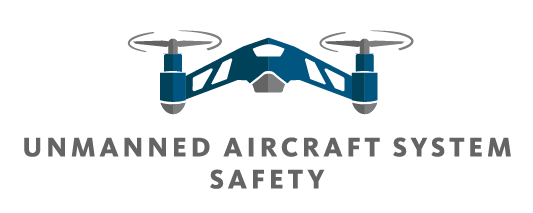
\includegraphics{COE_logo} \end{center}

The \textbf{UC Center of Excellence on Unmanned Aircraft System Safety} provides the following non-binding guidance to assist in the implementation of the Presidential Unmanned Aircraft System Policy (Policy), including the management of UAS Activity at University ocations and the development of Location Specific Policies or Procedures regarding the use of UAS at University locations.

The guidance is intended to 1) elaborate on the current regulatory environment and compliance requirements, 2) describe suitable means of compliance with the UC UAS Policy and 3) provide example language that may be used in location specific policy or procedures or in communication.

To the extent of any inconsistencies between the minimum requirements set in the UC UAS Policy or this guidance document and any applicable regulation, the regulatory requirements govern.

\begin{quote}
This document is expected to continue to be revised and updated regularly as a result of regulatory changes, improvements to safety best practices and user feedback.

Address comments to \href{mailto:UASSafety@ucmerced.edu}{\nolinkurl{UASSafety@ucmerced.edu}}
\end{quote}

\newpage

\hypertarget{revision-history}{%
\chapter*{Revision History}\label{revision-history}}
\addcontentsline{toc}{chapter}{Revision History}

\begin{longtable}[]{@{}lll@{}}
\toprule
Date & Rev & Notes\tabularnewline
\midrule
\endhead
2018/01/26 & 1.0 & Initial Document\tabularnewline
2018/07/01 & 1.1 & Revision\tabularnewline
2020/07/01 & 2.0 & Moved Online\tabularnewline
\bottomrule
\end{longtable}

\hypertarget{ch_policy}{%
\chapter{The Presidential UAS Policy}\label{ch_policy}}

The purpose of the University of California (UC) Presidential Policy on \protect\hyperlink{UAS}{Unmanned Aircraft Systems} is to establish minimum standards for the safe use and operation of \protect\hyperlink{UAS}{Unmanned Aircraft System} and \protect\hyperlink{sUAS}{Small Unmanned Aircraft System}, including drones and model aircraft, on any \protect\hyperlink{UL}{University Location} or for any \protect\hyperlink{UB}{University Business}. The Policy requires that all \protect\hyperlink{UAS}{UAS} operations are performed in a manner that mitigates risk to safety, security and privacy, and ensures compliance with any applicable regulation. A copy of the text of the Policy can be found in Section.

The scope of the policy includes:

\begin{itemize}
\tightlist
\item
  The operation of any \protect\hyperlink{UA}{Unmanned Aircraft} owned by the UC.
\item
  The operation of any \protect\hyperlink{UA}{Unmanned Aircraft} at or within the property owned or managed by the UC.
\item
  The operation of any \protect\hyperlink{UA}{Unmanned Aircraft} used for \protect\hyperlink{UB}{University Business}.
\end{itemize}

The Policy is summarized as below:

\begin{itemize}
\tightlist
\item
  The Policy establishes a \protect\hyperlink{SDA}{Systemwide Designated UAS Authority}.
\item
  The Policy establishes the development of a UAS Advisory Board.
\item
  The Policy establishes that an Executive Officer of a \protect\hyperlink{UL}{University Location} may appoint a \protect\hyperlink{DLA}{Designated Local Authority}.
\item
  The Policy establishes that an Executive Officer of a \protect\hyperlink{UL}{University Location} may authorize the development and implementation of \protect\hyperlink{LSP}{location specific policies or procedures} at any \protect\hyperlink{UL}{University Location} within the Executive Officer's jurisdiction.
\item
  The Policy establishes that anyone who seeks to operate a UAS under the jurisdiction of this policy must:

  \begin{itemize}
  \tightlist
  \item
    Comply with any applicable regulation.
  \item
    Have prior approval from a \protect\hyperlink{DLA}{Designated Local Authority} or \protect\hyperlink{SDA}{Systemwide Designated UAS Authority}.
  \item
    Operate in a manner that ensures public safety, right to privacy, civil rights and civil liberties.
  \item
    Maintain sufficient liability insurance coverage.
  \end{itemize}
\item
  All UAS activity under this Policy must be documented and reported.
\item
  All UC-owned UAS must be properly registered to the UC and submitted to the \protect\hyperlink{DLA}{Designated Local Authority} or \protect\hyperlink{SDA}{Systemwide Designated UAS Authority}.
\item
  Registration documents for UAS used for \protect\hyperlink{UB}{University Business} must be submitted to the \protect\hyperlink{DLA}{Designated Local Authority} or \protect\hyperlink{SDA}{Systemwide Designated UAS Authority}.
\item
  All UAS activity must have aviation liability coverage.
\item
  All UAS activity foreign nations or by foreign nationals must follow export control regulations and the UC Export Control Policy.
\end{itemize}

\hypertarget{role-of-the-presidential-uas-policy}{%
\section{Role of the Presidential UAS Policy}\label{role-of-the-presidential-uas-policy}}

The use of UAS is very nuanced across the wide diversity of use and few static generalizations regarding standards are appropriate. The Policy is intended to be flexible and adaptive to a wide range of needs. It is not intended for direct implementation for end-users, rather it is intended for a \protect\hyperlink{UL}{University Location} to aid in the oversight and management of UAS by setting uniform minimum compliance standards and in the establishment of a \protect\hyperlink{DLA}{Designated Local Authority} to provide services at the end-user level, department level, campus level and system level.

The value of the Policy is in the structure of the management of UAS activity. By establishing a common process and listing out roles and responsibilities, the Policy provides the UC system with:

\begin{itemize}
\tightlist
\item
  Access to UAS subject matter experts.
\item
  Standardized interpretation of UAS related regulations.
\item
  Ability to share best practices across campuses.
\item
  Transparency and accountability on UAS activity.
\item
  Transparency and accountability on UAS activity request reviews.
\end{itemize}

\hypertarget{role-of-the-systemwide-designated-authority}{%
\section{Role of the Systemwide Designated Authority}\label{role-of-the-systemwide-designated-authority}}

The role of the \protect\hyperlink{SDA}{Systemwide Designated UAS Authority} is defined as

\begin{itemize}
\tightlist
\item
  Provides interpretation of UAS regulations.
\item
  Develops internal University policies on certification and flight safety training.
\item
  Reviewing and approving applications for operation of UAS at a \protect\hyperlink{UL}{University Location} or for \protect\hyperlink{UB}{University Business}.
\item
  Maintains a record of all UAS activity within the scope of the Policy.
\item
  Ensures Policy compliance with applicable laws and regulations.
\item
  Tracks and manages the University response to pending and upcoming UAS legislation, regulations, policies and guidances.
\end{itemize}

\hypertarget{role-of-the-uas-advisory-board}{%
\section{Role of the UAS Advisory Board}\label{role-of-the-uas-advisory-board}}

The \protect\hyperlink{AB}{UAS Advisory Board} is responsible for:

\begin{itemize}
\tightlist
\item
  Reviewing exemptions from the Policy.
\item
  Assisting in the development of systemwide UAS policies.
\item
  Reviewing and commenting on proposed policies and long-term goals.
\item
  Evaluating the effectiveness of systemwide UAS policies and safety metrics.
\item
  Ensuring that systemwide UAS policies remain consistent with applicable privacy best practices (See Section).
\end{itemize}

Active areas of discussion for the \protect\hyperlink{AB}{UAS Advisory Board} are anticipated to include:

\begin{itemize}
\tightlist
\item
  Guidance and standards on \protect\hyperlink{LSP}{location specific policy or procedure}.
\item
  Proposed UAS regulations on UAS activity above non-participating persons.
\item
  Proposed UAS regulations related to UAS delivery services.
\item
  Counter-UAS technology deployment and use.
\item
  Delivery services.
\end{itemize}

\hypertarget{uas-activity-not-included-in-the-scope-of-the-systemwide-policy}{%
\section{UAS Activity not included in the Scope of the Systemwide Policy}\label{uas-activity-not-included-in-the-scope-of-the-systemwide-policy}}

UAS Activity not covered within the scope of the Policy:

\begin{itemize}
\tightlist
\item
  Personally-owned \protect\hyperlink{UA}{Unmanned Aircraft} not used at a \protect\hyperlink{UL}{University Location}.
\item
  Personally-owned \protect\hyperlink{UA}{Unmanned Aircraft} used for coursework (See Section ) and not used at a \protect\hyperlink{UL}{University Location}
\item
  Student club-owned \protect\hyperlink{UA}{Unmanned Aircraft} not used at a \protect\hyperlink{UL}{University Location}
\end{itemize}

The use of UAS by Emergency First Responders may additionally be exempt as necessary. However, any use of UAS by Emergency First Responders must follow their internal department protocols.

\hypertarget{relation-of-uc-systemwide-uas-policy-with-existing-ucop-policies}{%
\section{Relation of UC Systemwide UAS Policy with Existing UCOP Policies}\label{relation-of-uc-systemwide-uas-policy-with-existing-ucop-policies}}

All efforts have been made to ensure that the Policy is congruent with existing UCOP policies.

Examples of congruence with existing UCOP policies:

\begin{itemize}
\tightlist
\item
  \href{https://www.ucop.edu/academic-personnel-programs/academic-personnel-policy/policy-issuances-and-guidelines/revised-apm-015-and-016.html}{APM 015-016} addresses the Faculty Code of Contact and the administration of discipline in regards to policy non-compliance.
\item
  \href{https://www.ucop.edu/academic-personnel-programs/academic-personnel-policy/general-university-policy-regarding-academic-appointees/index.html}{APM 150-160} addresses Non-Senate Academic Appointees Grievances and Corrective Actions in regards to policy non-compliance.
\item
  \href{http://policy.ucop.edu/doc/3220476}{BFB-BUS-19: Registration and Licensing of University-Owned Vehicles} addresses registration and requires that all motor vehicles, aircraft and watercraft shall be registered on behalf of the University by the designated University location representative and the designated University location representative ensures governmental compliance.
\item
  \href{http://policy.ucop.edu/doc/3220477}{BFB-BUS-29:Management and Control of University Equipment} establishes the requirements of management and control of UC equipment.
\item
  \href{http://policy.ucop.edu/doc/3520505}{BFB-BUS-81: Insurance Programs} establishes that the University purchases aviation insurance to provide coverage for liabilities arising from the University's aviation operations that result in bodily injury and/or property damage.
\item
  \href{http://policy.ucop.edu/doc/2710521}{PACAOS-14: Definitions} establishes common definitions used in Policies Applying to Campus Activities, Organizations and Students (PACAOS), including definitions of `Campus', `Property' and `University'.
\item
  \href{http://policy.ucop.edu/doc/2710523}{PACAOS-30: Policy on Speech and Advocacy} establishes that the University is committed to assuring that all persons may exercise their constitutional rights.
\item
  \href{http://policy.ucop.edu/doc/2710524}{PACAOS-40: Policy on Use of University Properties} establishes the policy on the use of University properties that provides the basis for oversight.
\item
  \href{https://policy.ucop.edu/doc/2710530/PACAOS-100}{PACAOS-100.00 Policy on Student Conduct and Discipline} addresses policy non-compliance for students and visitors to a \protect\hyperlink{UL}{University Location}.
\item
  \href{https://policy.ucop.edu/manuals/personnel-policies-for-staff-members.html}{PPSM 62-65} addresses policy non-compliance for employees and staff members of the UC.
\item
  \href{http://policy.ucop.edu/doc/3500506}{Management of Health, Safety and the Environment} states that all University Activities are to be conducted in a manner than ensures the protection of students, faculty, staff, visitors, the public, property and the environment.
\item
  \href{https://policy.ucop.edu/doc/1100171/Whistleblower}{Policy on Reporting and Investigating Allegations of Suspected Improper Governmental Activities} addresses the responsibility of the UC to detect, prevent or deter improper activities.
\item
  \href{https://policy.ucop.edu/doc/2000676/ECP}{Export Control Policy} addresses requirements for export controlled equipment (including UAS) and their use internationally and by foreign nationals.
\end{itemize}

\hypertarget{ch_campus}{%
\chapter{Campus or Medical Center Authority}\label{ch_campus}}

Campus and Medical Center \protect\hyperlink{EO}{Executive Officer} (or their designees) may elect to appoint a \protect\hyperlink{DLA}{Designated Local Authority} and to authorize the development and implementation of \protect\hyperlink{LSP}{location specific policies or procedures}.

As many \protect\hyperlink{UL}{University Location} have experienced, \protect\hyperlink{UAS}{UAS} activity is diverse. Documented \protect\hyperlink{UASactivity}{UAS activity} have included:

\begin{itemize}
\tightlist
\item
  Engineering coursework -- Indoors and Outdoors
\item
  On-campus UAS research flights
\item
  Fieldwork within the \protect\hyperlink{NRS}{UC Natural Reserve System}
\item
  Fieldwork on private property
\item
  Research projects at \protect\hyperlink{ANR}{UC Division of Agriculture and Natural Resources} Research and Extension Centers
\item
  Student \protect\hyperlink{drone}{drone} clubs and student recreation
\item
  Campus Media and Strategic Communications
\item
  Facility Management and Construction Monitoring
\item
  (ref:3rdParty) Contractors
\item
  (ref:3rdParty) Film Crews
\end{itemize}

Even within similar purposes and locations, different risk factors may lead to drastically different \protect\hyperlink{riskscore}{Risk Score}. It is strongly recommended that \protect\hyperlink{UL}{University Location} develop a \protect\hyperlink{LSP}{location specific policy or procedure} that can scale appropriately.

\hypertarget{sec_LSP}{%
\section{Location-Specific Policy}\label{sec_LSP}}

Each Campus and Medical Center is encouraged to develop a \protect\hyperlink{LSP}{location specific policy or procedure} to address local issues.

A \protect\hyperlink{LSP}{location specific policy or procedure} may include but is not limited to addressing the following questions:

\begin{itemize}
\tightlist
\item
  Who approves flights for the location?
\item
  Will departments or subgroups have the autonomy to approve flights with consultation from the \protect\hyperlink{DLA}{Designated Local Authority}?
\item
  Who should be notified regarding on-campus UAS activity?
\item
  What are the terms of approval?
\item
  Who has priority to operate a UAS?
\item
  Specific areas where UAS activity is prohibited
\item
  Availability of areas where UAS activity may be operated recreationally
\item
  How long an approval may be valid?
\item
  Enforcement of UAS policies
\item
  Creation of a UAS committee or working group to advice local policies
\item
  Procedures regarding the purchase of a UAS
\item
  Standards regarding privacy
\end{itemize}

A Campus or Medical Center may elect to not develop a location-specific policy, in which the \protect\hyperlink{DLA}{Designated Local Authority} (if appointed) or \protect\hyperlink{SDA}{Systemwide Designated UAS Authority} (if no \protect\hyperlink{DLA}{Designated Local Authority} is appointed) may review and approve \protect\hyperlink{UASactivity}{UAS activity} on a case-by-case basis.

\hypertarget{sec_DLA}{%
\section{Designated Local Authority}\label{sec_DLA}}

The \protect\hyperlink{DLA}{Designated Local Authority} is a local authority that serves as a single point of contact for \protect\hyperlink{UASactivity}{UAS activity} for a \protect\hyperlink{UL}{University Location}. This single point of contact serves as a means to funnel UAS inquiries, including purchasing and \protect\hyperlink{FR}{Flight Request}, across the \protect\hyperlink{UL}{University Location} for standardized information and interpretations.

The responsibilities of a \protect\hyperlink{DLA}{Designated Local Authority} may additionally be delegated and shared across multiple departments as long as there remains a focal point for coordination and records.

\hypertarget{example-roles-responsibilities}{%
\subsection{Example Roles \& Responsibilities}\label{example-roles-responsibilities}}

\begin{itemize}
\tightlist
\item
  Is responsible for regulatory compliance and risk management of \protect\hyperlink{UASactivity}{UAS activity} within their authority.
\item
  Maintains a list of UAS \protect\hyperlink{UASactivity}{UAS activity}.
\item
  Coordinates \protect\hyperlink{UASactivity}{UAS activity} across multiple departments for appropriate reviews.
\item
  Ensures UAS liability insurance coverage for all activity.
\item
  Reviews and interprets applicable regulations and policies at the campus-level.
\item
  Serve as the liaison between regulatory agencies and the operators.
\end{itemize}

As many \protect\hyperlink{DLA}{Designated Local Authority} are housed in Environmental Health \& Safety or Risk Management departments, they may also fulfill additional roles expected of those departments.

\begin{itemize}
\tightlist
\item
  Provide consultation on \protect\hyperlink{UASactivity}{UAS activity} - safe flying locations, hazard analysis, equipment use.\\
\item
  Provide flight instruction.
\item
  Conduct lab or field safety audits.
\item
  Remedy faults and remediates poor safety training.
\end{itemize}

\hypertarget{congruence-with-existing-campus-policies}{%
\section{Congruence with Existing Campus Policies}\label{congruence-with-existing-campus-policies}}

Any \protect\hyperlink{UASactivity}{UAS activity} on a \protect\hyperlink{UL}{University Location} must comply with any existing policy or procedure. As \protect\hyperlink{UASactivity}{UAS activity} is a new and growing trend, it is not uncommon that a proponent is unfamiliar with the breadth of existing policies.

Some common policies to review for

\begin{itemize}
\tightlist
\item
  Delegation of Authority
\item
  Policy on Use and Scheduling Properties
\item
  Policy on Filming and Photography
\item
  Materiel Management and Property Inventory Control
\item
  Policy on Lab Safety
\item
  Policy on Field Safety
\item
  Privacy Policies
\item
  Use of UC Managed Reserves or Field Stations
\item
  Campus Recreation and Facilities
\item
  Police Authority and Jurisdiction
\end{itemize}

An effective \protect\hyperlink{LSP}{location specific policy or procedure} would include ssteps to ensure compliance with any applicable existing policy through an agreed upon process with any relevant authorities.

\hypertarget{ch_registration}{%
\chapter{Registration of UAS}\label{ch_registration}}

Within the US, all UA must be registered under the regulations specified by 14 CFR 47 or 14 CFR 48, depending on the weight of the aircraft, location of the aircraft's operation or primary purpose of the aircraft. Aircraft flown exclusively outside the US or within military airspace may be subject to other registration requirements.

\hypertarget{registration-of-uc-owned-uas}{%
\section{Registration of UC-owned UAS}\label{registration-of-uc-owned-uas}}

The Regents are the legal owners of all UC property. Similarly to BFB-BUS-19: Registration and Licensing of University-Owned Vehicles, all UC-owned UA must be registered to the Regents () to meet compliance obligations under 14 CFR 47 or 14 CFR 48.

\begin{center}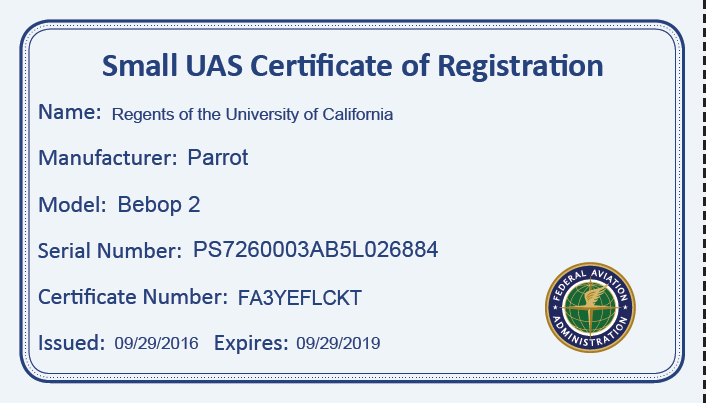
\includegraphics{reg_cert} \end{center}

Registration under 14 CFR 48 may be done online () at \url{https://faadronezone.faa.gov/}.

UAS that weigh more than 55 lbs or are required to have UAS registration that is valid internationally must be registered under 14 CFR 47 and must be done through mail with an Original Aircraft Registration Form, AC Form 8050-1.

\hypertarget{registration-of-model-aircraft}{%
\section{Registration of Model Aircraft}\label{registration-of-model-aircraft}}

Model Aircraft are required to be registered under 14 CFR 48. Though typically most UAS owned by the UC will be registered individually, there are some cases where they may be registered as MA.

\begin{quote}
In general, UAS that are used exclusively as model aircraft may be registered as a group under the owner of the model aircraft. In the case of the group or company owned model aircraft, they may be registered under the primary user or manager of the model aircraft as the model aircraft registration is not considered proof of ownership.
\end{quote}

\textbf{Common Scenarios for Model Aircraft}

\begin{itemize}
\tightlist
\item
  Model Aircraft owned by students should be registered by the student
\item
  Model Aircraft owned by a student club can be registered by a member of the student club, a club mentor or faculty advisor.
\item
  Model Aircraft used in classroom or educational activity should have the faculty, instructor or department staff member register for an FAA registration number to be placed on all aircraft.
\end{itemize}

\hypertarget{record-keeping-policy-requirements}{%
\section{Record Keeping Policy Requirements}\label{record-keeping-policy-requirements}}

Records of UC-owned UAS registration must be provided to the designated local authority or the systemwide designated authority. Registration of all unmanned aircraft used for University business must be provided to the designated local authority or the systemwide designated authority. UC Drones may be used to submit records electronically and other electronic submission processes may be available in the future. A University location may additionally implement a centralized registration process using a single FAA online account.

\hypertarget{applications}{%
\chapter{Applications}\label{applications}}

Some \emph{significant} applications are demonstrated in this chapter.

\hypertarget{example-one}{%
\section{Example one}\label{example-one}}

\hypertarget{example-two}{%
\section{Example two}\label{example-two}}

\hypertarget{glossary}{%
\chapter{Glossary}\label{glossary}}

\hypertarget{rdparty}{%
\subsubsection*{\texorpdfstring{3\textsuperscript{rd} Party}{3rd Party}}\label{rdparty}}
\addcontentsline{toc}{subsubsection}{3\textsuperscript{rd} Party}

For the purposes of this document, a \protect\hyperlink{rdparty}{3\textsuperscript{rd} Party} is defined as any person who is conducting \protect\hyperlink{UB}{University Business} but is not affiliated with the UC or any person not conducting \protect\hyperlink{UB}{University Business}.



\hypertarget{DLA}{%
\subsubsection*{Designated Local Authority}\label{DLA}}
\addcontentsline{toc}{subsubsection}{Designated Local Authority}

The \protect\hyperlink{DLA}{Designated Local Authority} is a single-point of contact or committee appointed by an \protect\hyperlink{EO}{Executive Officer} at an individual \protect\hyperlink{UL}{University Location} to oversee the development, implementation, and enforcement of any University Location-specific UAS related policies and procedures.



\hypertarget{drone}{%
\subsubsection*{Drone}\label{drone}}
\addcontentsline{toc}{subsubsection}{Drone}

The term \protect\hyperlink{drone}{drone} is a colloquoal or common tsynonymous with \protect\hyperlink{UAS}{Unmanned Aircraft System}.



\hypertarget{EO}{%
\subsubsection*{Executive Officer}\label{EO}}
\addcontentsline{toc}{subsubsection}{Executive Officer}

The \protect\hyperlink{EO}{Executive Officer} means any of the University of California's Chancellors, Medical Center Chief Executive Officers, Director of Lawrence Berkeley National Laboratory, and Vice President for Agriculture and Natural Resources.



\hypertarget{FR}{%
\subsubsection*{UAS Request Form}\label{FR}}
\addcontentsline{toc}{subsubsection}{UAS Request Form}

The term \protect\hyperlink{FR}{UAS Request Form} or \protect\hyperlink{FR}{Flight Request} refers to a documented request to operate a UAS pursuant to this Policy. The Policy does not mandate a specific form or system as long as the minimum review criteria is met. See Section () for further details.





\hypertarget{LSP}{%
\subsubsection*{Location Specific Policy or Procedure}\label{LSP}}
\addcontentsline{toc}{subsubsection}{Location Specific Policy or Procedure}

The term \protect\hyperlink{LSP}{location specific policy or procedure} means a policy or procedure, or a set of policies or procedures, established at a \protect\hyperlink{UL}{University Location}. The policy or procedure must include a review as described in Section (), but may be flexible to address a diverse set of \protect\hyperlink{UASactivity}{UAS activity}.





\hypertarget{riskscore}{%
\subsubsection*{Risk Score}\label{riskscore}}
\addcontentsline{toc}{subsubsection}{Risk Score}

For the purposes of this document, the term \protect\hyperlink{riskscore}{Risk Score} refers to a customized Risk Score between 1-5 that communicates an approximately level of risk; ranging from minor to severe (potential to cause injury or significant property damage). See Section () for a description of the \protect\hyperlink{riskscore}{Risk Score} and scoring matrix.



\hypertarget{sUAS}{%
\subsubsection*{Small Unmanned Aircraft System}\label{sUAS}}
\addcontentsline{toc}{subsubsection}{Small Unmanned Aircraft System}

The term \protect\hyperlink{sUAS}{Small Unmanned Aircraft System} means an \protect\hyperlink{UA}{Unmanned Aircraft} weighing less than 55 lbs. and associated elements that are required to operate safely and efficiently in the national airspace system.





\hypertarget{SDA}{%
\subsubsection*{Systemwide Designated UAS Authority}\label{SDA}}
\addcontentsline{toc}{subsubsection}{Systemwide Designated UAS Authority}

The term \protect\hyperlink{SDA}{Systemwide Designated UAS Authority} refers to the authority appointed by the University of California Office of the President (UCOP) Environment, Health \& Safety (EH\&S) Executive Director. The responsibilites of the \protect\hyperlink{SDA}{Systemwide Designated UAS Authority} include providing interpretation of \protect\hyperlink{UAS}{UAS} regulations, developing \protect\hyperlink{UAS}{UAS} policies and procedures, maintaining records of all \protect\hyperlink{UASactivity}{UAS activity} and ensuring regulatory compliance.



\hypertarget{ANR}{%
\subsubsection*{UC Agriculture and Natural Resources}\label{ANR}}
\addcontentsline{toc}{subsubsection}{UC Agriculture and Natural Resources}

The \protect\hyperlink{ANR}{UC Division of Agriculture and Natural Resources} (UC ANR) is a division of the University of California system that connects the power of UC research in agriculture, natural resources, nutrition, and youth development with local communities. UC ANR statewide programs includes 4-H, Cooperative Extensions, Master Gardener Program, and includes a system of Research and Extension Centers across California.



\hypertarget{NRS}{%
\subsubsection*{UC Natural Reserve System}\label{NRS}}
\addcontentsline{toc}{subsubsection}{UC Natural Reserve System}

The \protect\hyperlink{NRS}{UC Natural Reserve System} (UC NRS) is a system of protected ecosystems owned or managed by the University of California that is used for research, education, and public service. The reserves include examples of most of California's major habitat types, from grasslands and deserts to coastal wetlands and conifer forests. With more than 40 sites encompassing some 756,000 acres and growing, the UC NRS is the largest university-administered reserve system in the world.



\hypertarget{UB}{%
\subsubsection*{University Business}\label{UB}}
\addcontentsline{toc}{subsubsection}{University Business}

The term \protect\hyperlink{UB}{University Business} means the official activities of a University that contribute to any one of the University's major functions of teaching, research, patient care, or public service, or to any other non-recreational University purpose.



\hypertarget{UL}{%
\subsubsection*{University Location}\label{UL}}
\addcontentsline{toc}{subsubsection}{University Location}

Any property or building that is owned or leased by the University where University business or activities take place.



\hypertarget{UA}{%
\subsubsection*{Unmanned Aircraft}\label{UA}}
\addcontentsline{toc}{subsubsection}{Unmanned Aircraft}

The term \protect\hyperlink{UA}{Unmanned Aircraft} means an aircraft that is operated without the possibility of direct human intervention from within or on the aircraft. This definition includes aircraft of all sizes.





\hypertarget{UAS}{%
\subsubsection*{Unmanned Aircraft System}\label{UAS}}
\addcontentsline{toc}{subsubsection}{Unmanned Aircraft System}

The term \protect\hyperlink{UAS}{Unmanned Aircraft System} means an \protect\hyperlink{UA}{Unmanned Aircraft} and associated elements (including communication links and the components that control the unmanned aircraft) that are required for the pilot in command to operate safely and efficiently in the national airspace system. For the purposes of this Policy, this includes unmanned aircraft of all sizes and includes unmanned aircraft operated indoors, in military airspace or in foreign airspace systems.







\hypertarget{UASactivity}{%
\subsubsection*{UAS Activity}\label{UASactivity}}
\addcontentsline{toc}{subsubsection}{UAS Activity}

The term \protect\hyperlink{UASactivity}{UAS activity} refers to the act of flying for a defined purposed. It may be used to represent a single flight, a set of flights within a single day, a set of flights across multiple days, and may encompass multiple locations.



\hypertarget{AB}{%
\subsubsection*{UAS Advisory Board}\label{AB}}
\addcontentsline{toc}{subsubsection}{UAS Advisory Board}

The \protect\hyperlink{AB}{UAS Advisory Board} is created by the Policy for the purposes of reviewing and developing future \protect\hyperlink{UAS}{UAS} policies.



  \bibliography{book.bib,packages.bib}

\end{document}
